\documentclass[10pt]{article}

\usepackage[table,svgnames]{xcolor}
\usepackage{color}
\usepackage{hyperref}
\usepackage{graphicx}
\usepackage{multirow}
\usepackage{multicol}
\usepackage{tikz}
\usepackage{pgfplots}
\usetikzlibrary{shapes,arrows,matrix}
\usepackage{fancyhdr}
\usepackage{epigraph}
\usepackage{listings}
\usepackage{lastpage}
\usepackage{smartdiagram}
\usepackage{caption}
\usepackage{sectsty}

\definecolor{PCFTorange}{RGB}{145,34,5}
\definecolor{PCFTorangedark}{RGB}{79,26,12}
\definecolor{PCFTorangelight}{RGB}{255,96,62}

\allsectionsfont{\color{PCFTorangedark}}

\lstset{
  basicstyle=\small\ttfamily,
  keywordstyle=\color{blue},
  showstringspaces=false,
  frame=shadowbox,
  rulesepcolor=\color{PCFTorangedark},
  backgroundcolor=\color{PCFTorangelight},
  numberstyle=\small\color{gray},
  tabsize=2,
  numbers=left,
  breaklines=true,
  postbreak=\mbox{\textcolor{red}{$\hookrightarrow$}\space},
}

\lstdefinelanguage{lua}{
  morekeywords={
    function, local, return, end
 },
 keywordstyle=[2]{\textbf},
 morecomment=[l]{--},
 morestring=[b]{'},
 tabsize=4}

\title{\color{PCFTorangedark} \textbf{Pcraft Handbook\\ a companion to Pcraft}}
\author{Sebastien Tricaud $<$sebastien.tricaud@devo.com$>$\\
  Lead Developer of Pcraft\\
  \url{http://www.github.com/devoinc/pcraft}
}



%% Footer
\renewcommand{\footrulewidth}{0.4pt}
\cfoot{This is Pcraft Handbook. The Opensource crafting document released under MIT License.}



\begin{document}
\maketitle

\begin{center}
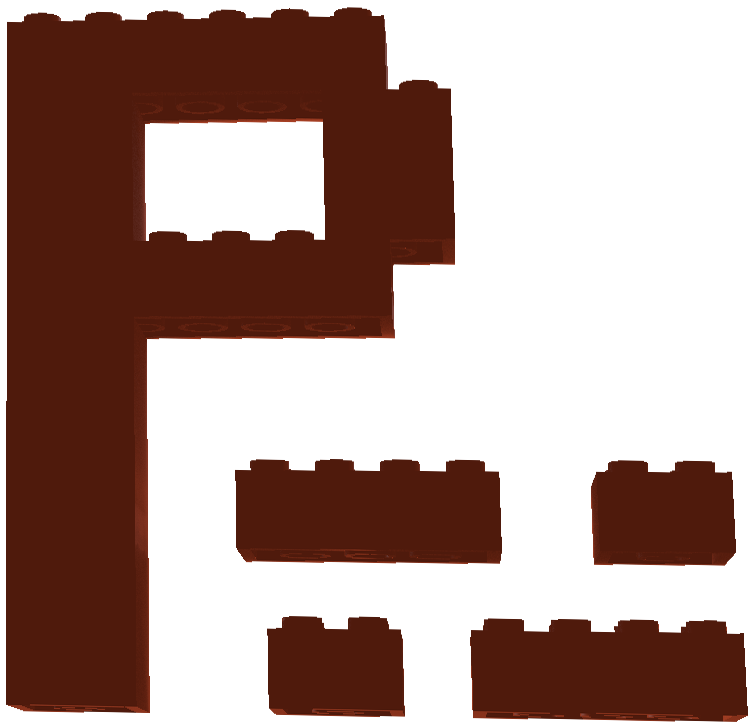
\includegraphics[width=4cm]{pcraft-logo.png}
\end{center}

\vspace{0.5in}

\begin{abstract}

\renewcommand{\epigraphflush}{center}
\begin{epigraphs}
\centering
\setlength{\epigraphwidth}{1.6\textwidth}
\qitem{Those are my principles, and if you don't like them... well, I have others.}{---\textsc{Groucho Marx}}
\end{epigraphs}

\vspace{1in}

Pcraft originally meant  ``Packet Crafter'', but now does much more! It is available from \url{http://www.github.com/devoinc/pcraft}. Pcraft will help you archive three things:
\begin{enumerate}
\item Create PCAPs from Scratch
\item Define Attack Scenarios
\item Write Logs for Simulated Devices
\end{enumerate}

\end{abstract}

{
\begin{figure}
\begin{center}
\caption{\textbf{Document Status}}
{\rowcolors{2}{PCFTorange}{PCFTorangelight}
\begin{tabular}{|c|l|l|}
\hline
\textbf{Date} & \textbf{Author} & \textbf{Description} \\
\hline
\today & Sebastien Tricaud & First version \\
\hline
\end{tabular}
}
\end{center}
\end{figure}
}

\newpage

\tableofcontents

\newpage

\section{Introduction}

This Handbook has one goal: help you learn Pcraft so anyone can use it and hack it.

\subsection{Cutting the Bla-bla}

This document is written to be the least boring possible. If you believe you can make one paragraph or section more fun to read, yet still communicating the point, I am more than welcoming Pull-Requests! A Handbook is not a complete boring manual. It is ready by your hand to search on how to do certains things. Like a cookbook, but hopefully you won't cook with Pcraft - QED.

\subsection{Creating named logs}


\section{Ami}

Ami is the language defined to help generating data correctly. It offers a way to describe actions, repeat loops, and how long does one sleep until the next action.

\subsection{Variables}

\subsection{Strings}

\subsection{Time}

\subsection{Loops}


\end{document}
